
\documentclass[aspectratio=169]{beamer}
\usetheme{metropolis}           % Use metropolis theme
\usepackage[utf8]{inputenc}
\usepackage{graphicx}
\usepackage{eso-pic}
\usepackage{graphics}
\usepackage{tikz}
\usepackage[export]{adjustbox}
\usepackage{multicol}
\usepackage{listings}
\usepackage{helvet}
\usepackage{booktabs}
\usepackage{threeparttable}


\title{Stata Coding for \newline Reproducible Research }
\date{\today}
\author{Benjamin Daniels} % Name of author(s) of session here
\institute{Development Impact Evaluation (DIME) \newline The World Bank }
\setbeamercolor{background canvas}{bg=white}	% Sets background color

% The below command places the World Bank logo and DIME logo to the right corner
\titlegraphic{%
	\begin{picture}(0,0)
	\put(330,-180){\makebox(0,0)[rt]{
\includegraphics[width=3cm]{img/WB_logo}}}
	\end{picture}%
	\begin{picture}(0,0)
	\put(390,-180){\makebox(0,0)[rt]{
\includegraphics[width=1.5cm]{img/i2i}}}
	\end{picture}%
}

%%% Section page with picture of Light bulb
\makeatletter
\defbeamertemplate*{section page}{mytheme}[1][]{
	\centering
	\begin{minipage}{22em}
		\raggedright
		\usebeamercolor[fg]{section title}
		\usebeamerfont{section title}
		\par
		\ifx\insertsubsectionhead\@empty\else%
		\usebeamercolor[fg]{subsection title}%
		\usebeamerfont{subsection title}%
		\fi
		\ifstrempty{#1}{}{%
			\includegraphics[width=100mm, height=60mm]{#1}%
		}
		\insertsectionhead\\[-1ex]
		\insertsubsectionhead
		\usebeamertemplate*{progress bar in section page}
		
	\end{minipage}
	\par
	\vspace{\baselineskip}
}
\makeatother

%%% Define a command to include picture in section, 
%%% make section, and revert to old template
\newcommand{\sectionpic}[2]{
	\setbeamertemplate{section page}[mytheme][#2]
	\section{#1}
	\setbeamertemplate{section page}[mytheme]
}

%%% The command below allows for the text that contains Stata code
\lstset{ %
	backgroundcolor=\color{white},
	basicstyle=\tiny,
	breakatwhitespace=false,
	breaklines=true,
	captionpos=b,
	commentstyle=\color{green},
	escapeinside={\%*}{*)},
	extendedchars=true,
	frame=single,
	numbers=left,
	numbersep=5pt,
	numberstyle=\tiny\color{gray},
	rulecolor=\color{black},
	showspaces=false,
	showstringspaces=false,
	showtabs=false,
	stringstyle=\color{mauve},
	tabsize=2,
	title=\lstname,
	morekeywords={not,\},\{,preconditions,effects },
	deletekeywords={time}
}

%% The below command creates the ligh bulb logos in the top right corner of the 
\begin{document}
	
{
	\usebackgroundtemplate{
\includegraphics[height=55mm, right]{img/top_right_corner.pdf}}
	\maketitle
}

%%%%%%%%%% heading of section 1 %%%%%%%%%%%%%%%%%%
\sectionpic{Introduction: Stata Coding}{img/section_slide}


\begin{frame}{Stata Coding}
\textbf{Stata coding is part of a reproducible research workflow:}

\begin{itemize}[<default overlay specification>]
	\item<1> It should be easy to read and re-adapt
	\item<1>  This means in terms of structure, syntax and style
	\item<1>  Code should be modularized as much as possible
	\item<1>  Anything that might be used again can be saved as an “adofile”
\end{itemize}
\end{frame}

\begin{frame}
	\begin{figure}
		\centering
		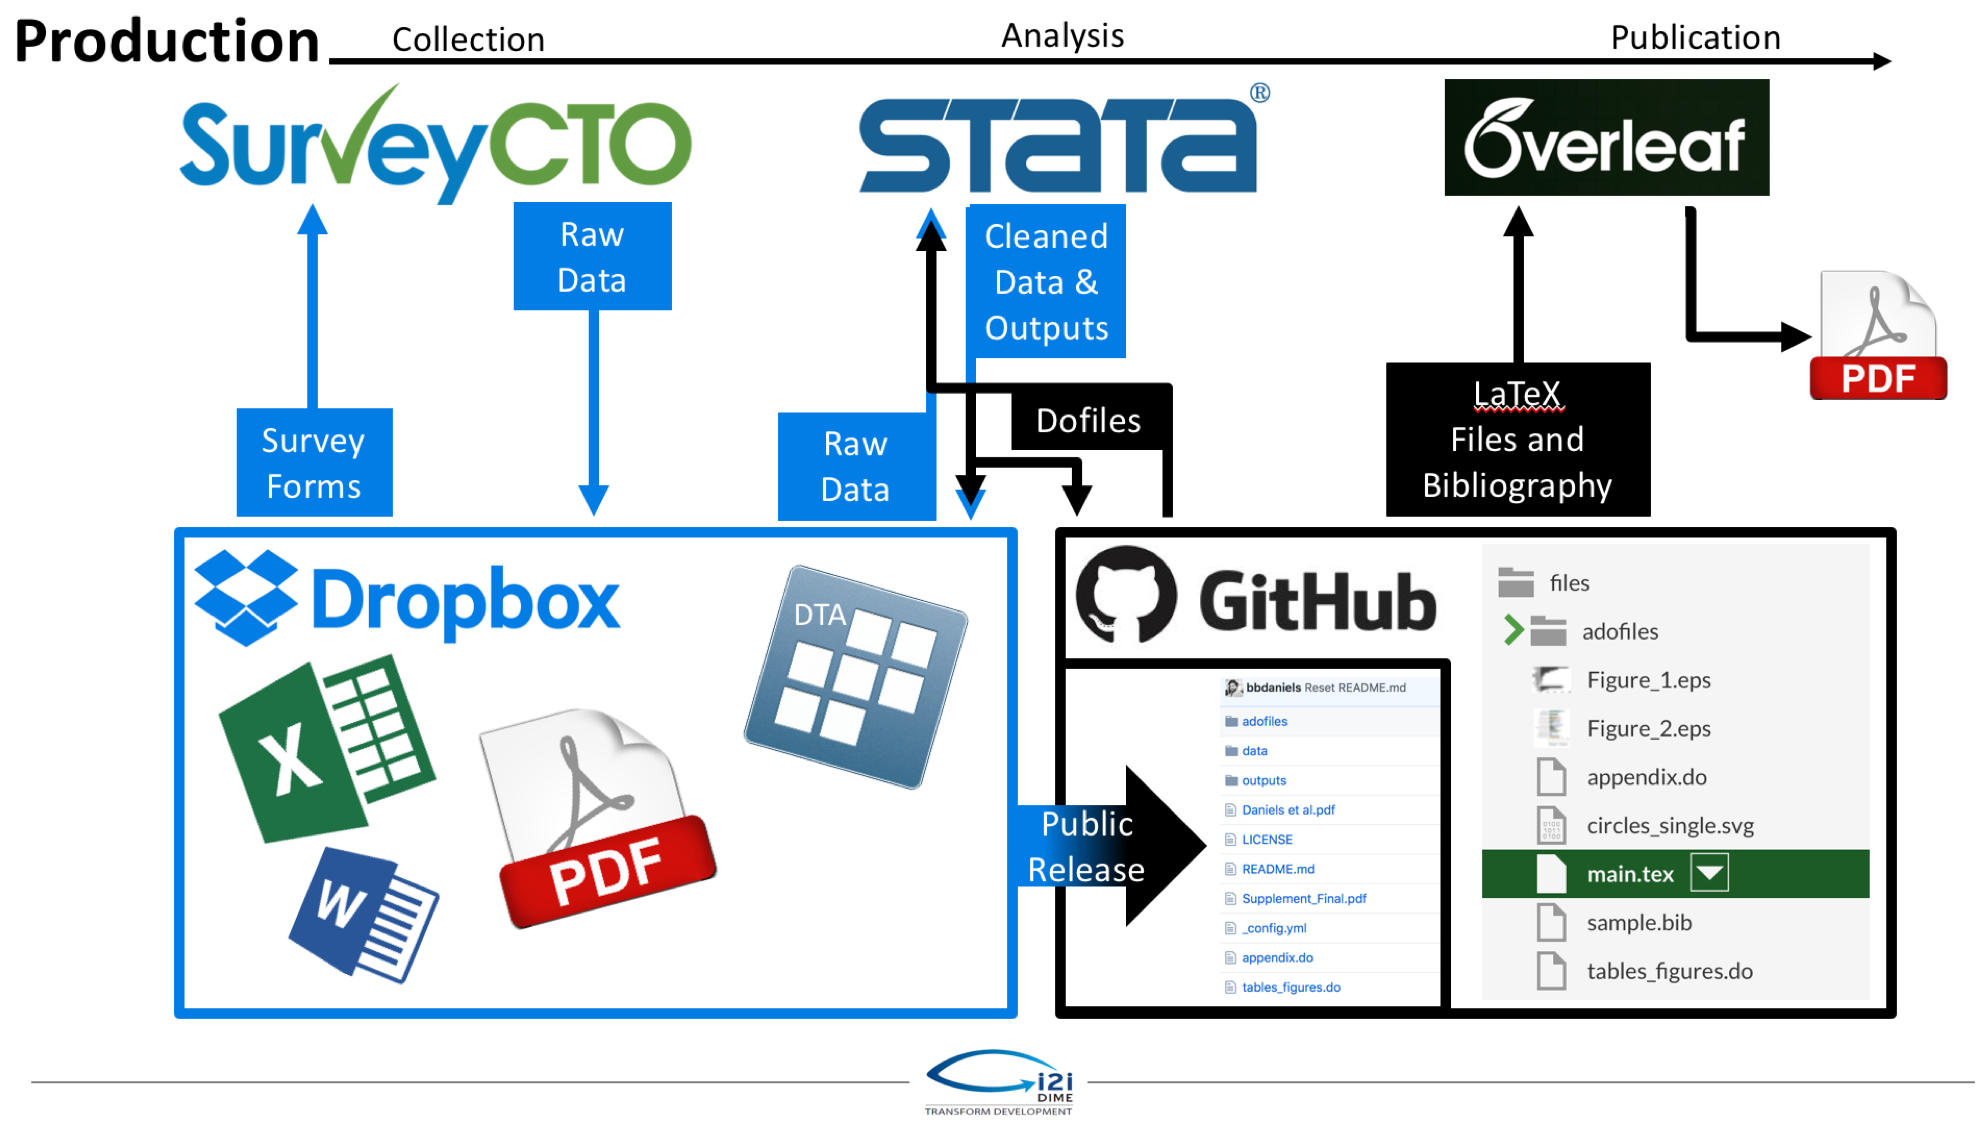
\includegraphics[width=\linewidth]{img/Production}
	\end{figure}
\end{frame}

%%%%%%%%%% heading of section 2 %%%%%%%%%%%%%%%%%%
\sectionpic{Stata Coding: Structure}{img/section_slide}

\begin{frame}{Coding Structure}
\begin{figure}
	\centering
	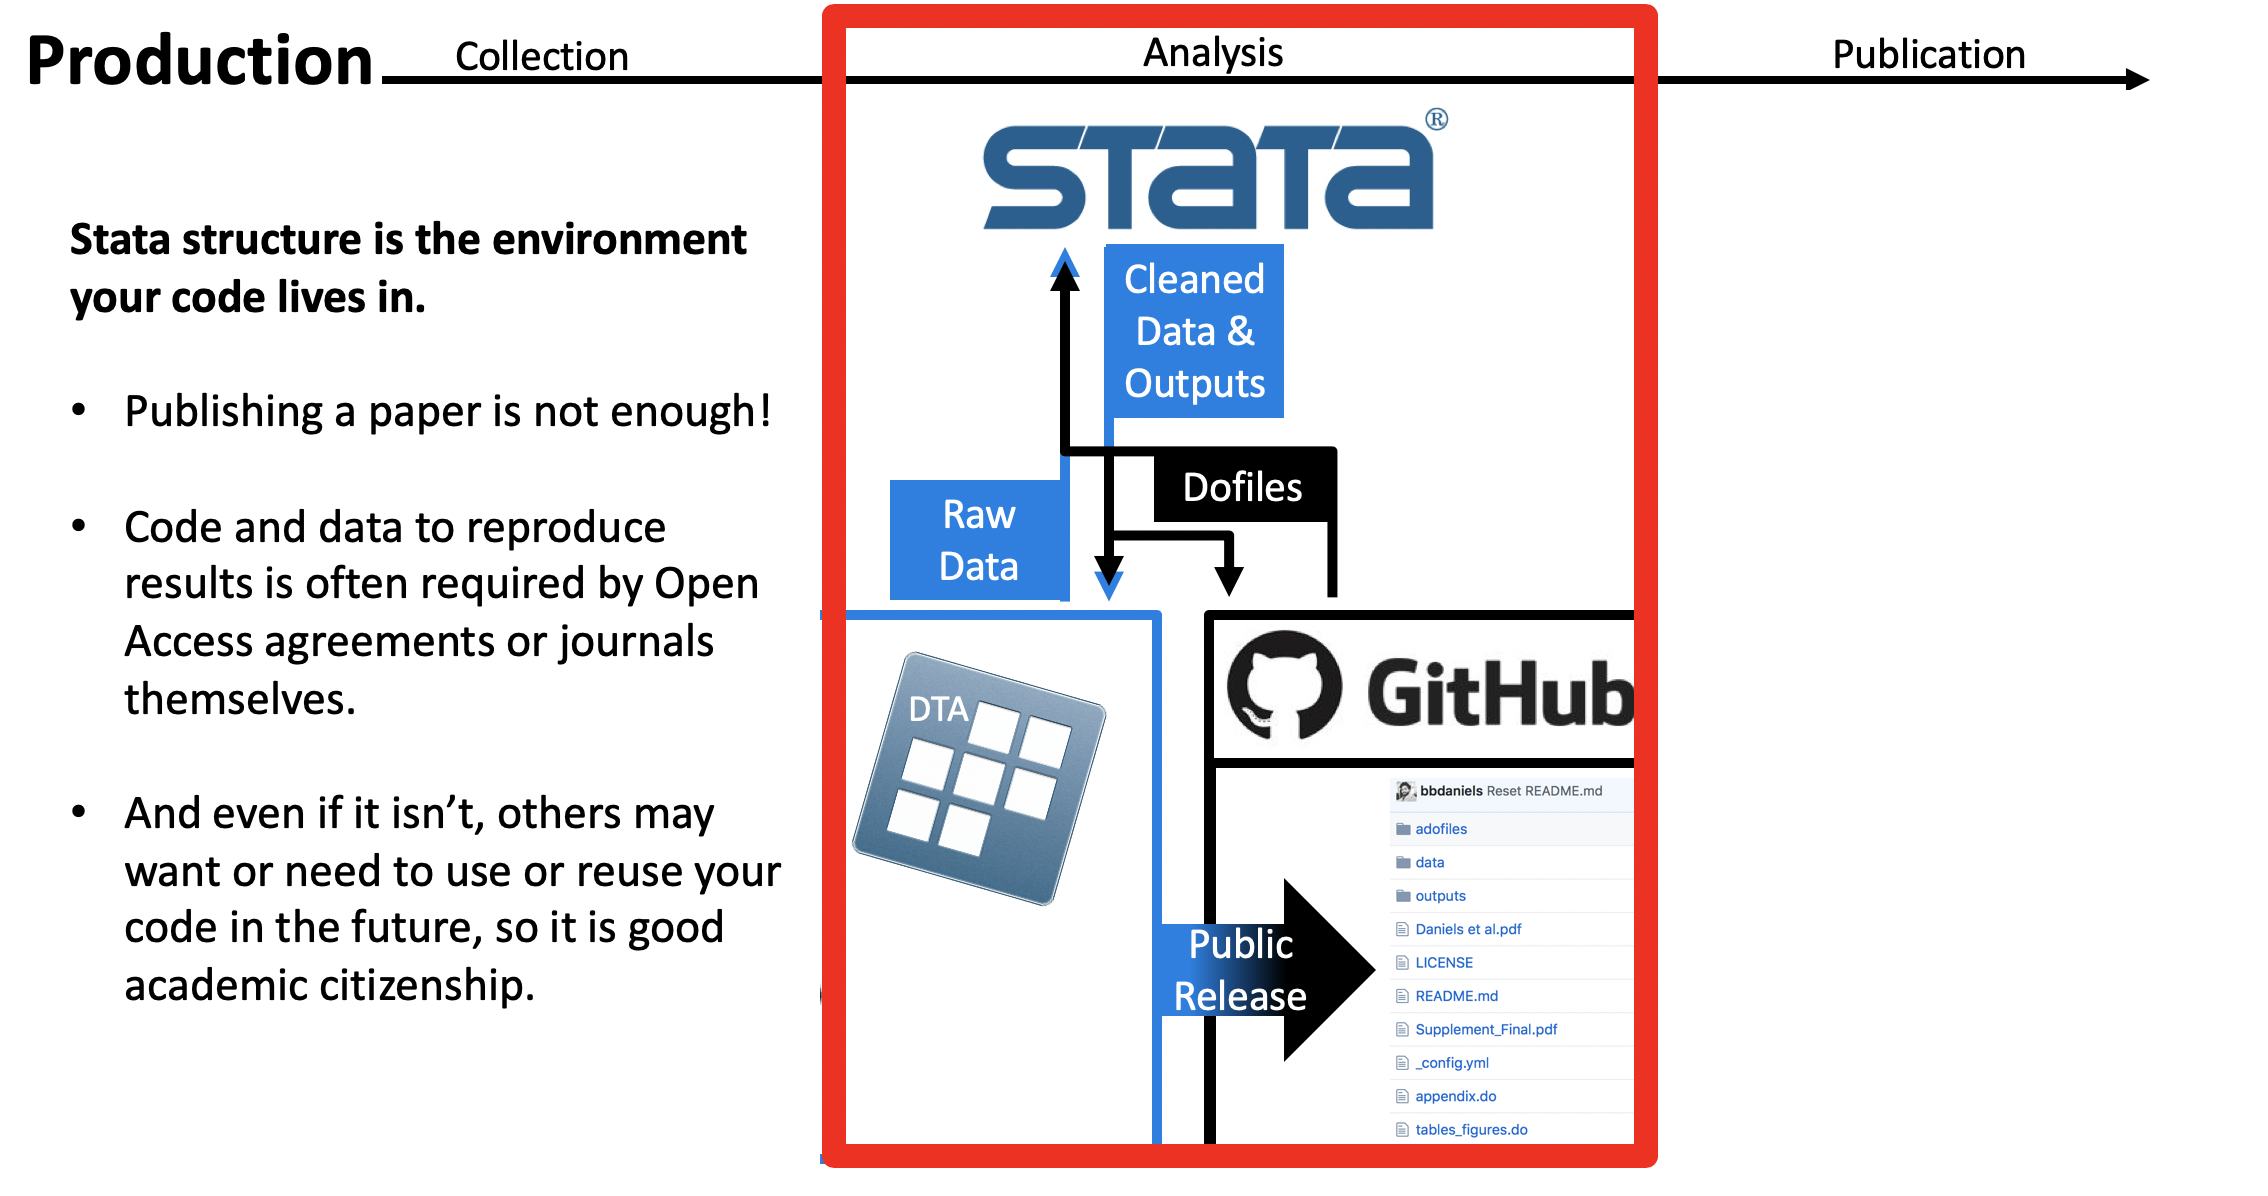
\includegraphics[width=\linewidth]{img/Production2}
\end{figure}
\end{frame}

\begin{frame}[fragile]{Modular organization is constant preparation}
\begin{multicols}{2}	
		
		\begin{itemize}[<default overlay specification>]
			\item<1> It is much easier to maintain files \textbf{modularly} from the outset than to clean up “everything dofiles”.
			\item<1>  Cleaning is \textbf{separated} from analysis so that each analysis step begins with [use].
			\item<1>  The final product then only consists of keeping the analysis files that are used in the paper and \textbf{archiving} the rest.
		\end{itemize}
	
		\begin{figure}
			\centering
			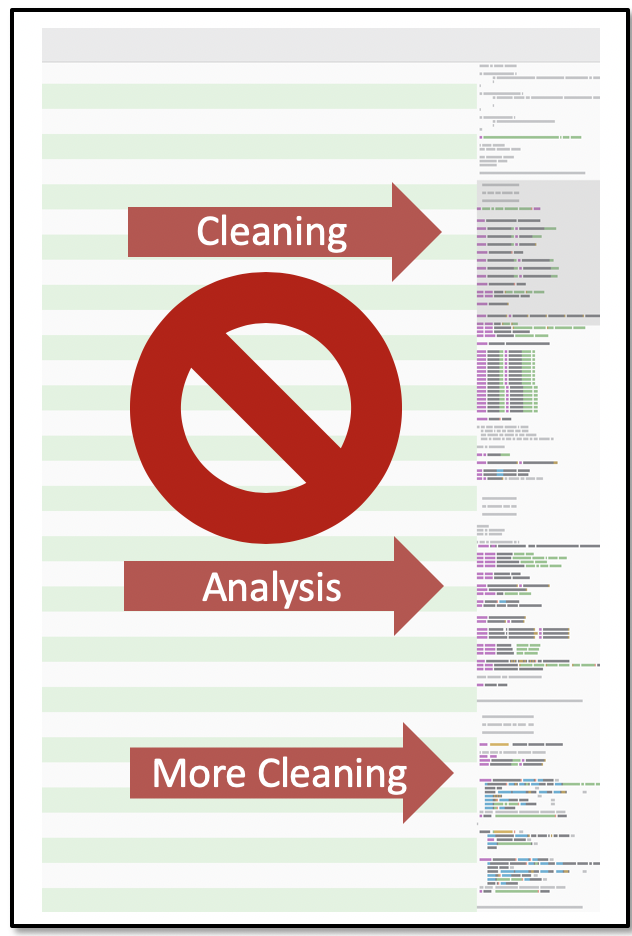
\includegraphics[width=50mm]{img/Structure}
		\end{figure}
	
\end{multicols}
\end{frame}

\begin{frame}{What does this look like in practice?}
\begin{figure}
	\centering
	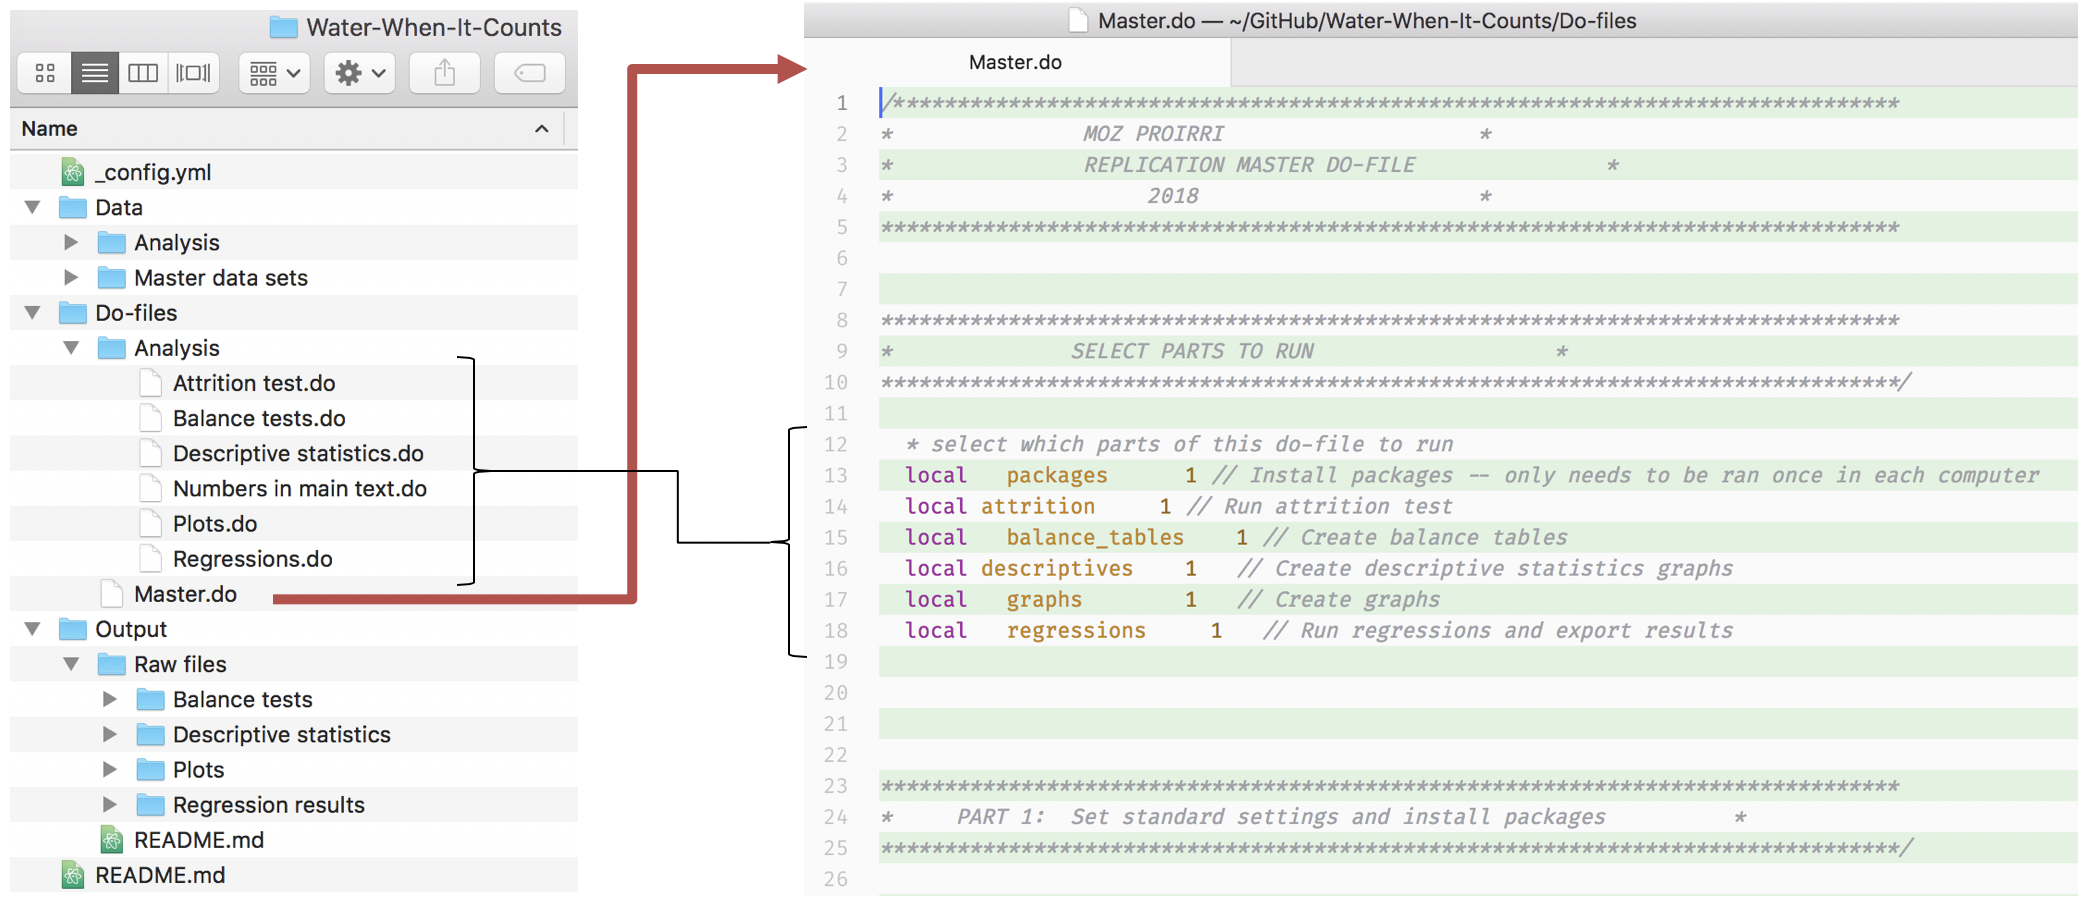
\includegraphics[width=\linewidth]{img/Structure2}
\end{figure}
\end{frame}


\begin{frame}[fragile]{Modular data analysis with Git(Hub)}
\begin{multicols}{2}	
	
	\begin{itemize}[<default overlay specification>]
		\item<1> Version Control –  Analysts can always find “that code that did that one thing”, and the current master version will have various experimental “branches” until they are confirmed functional and merged in.

		\item<1>  Efficiency – This allows simultaneous distributed editing of dofiles, text files, bibliographies, etc., but is not appropriate for Office/.dta/.pdf files.
		\item<1>  Privacy – Must use paid account (such as github.com/worldbank) to have “private” or “secret” folders. 
	\end{itemize}
	
	\begin{figure}
		\centering
		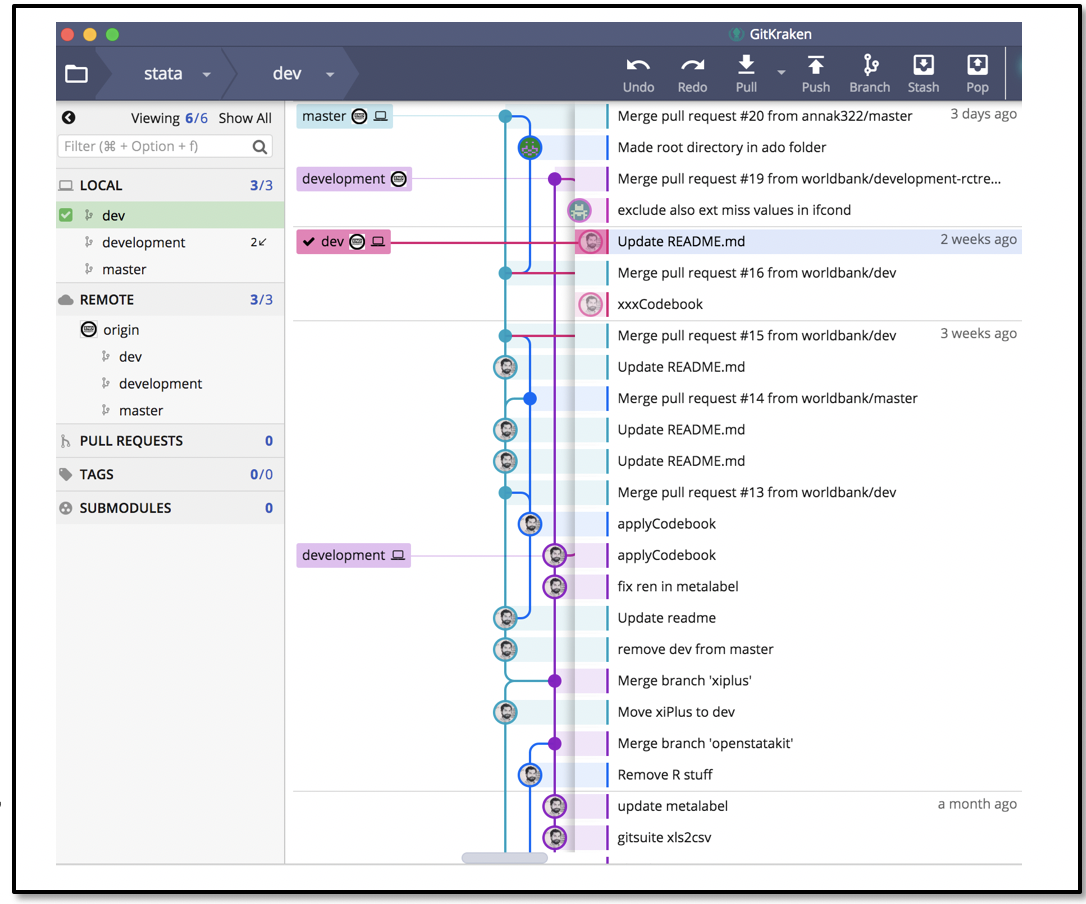
\includegraphics[width=65mm, right]{img/Structure3}
	\end{figure}
	
\end{multicols}
\end{frame}

\begin{frame}{Writing: LaTeX Documents (Overleaf + Git)}
\begin{figure}
	\centering
	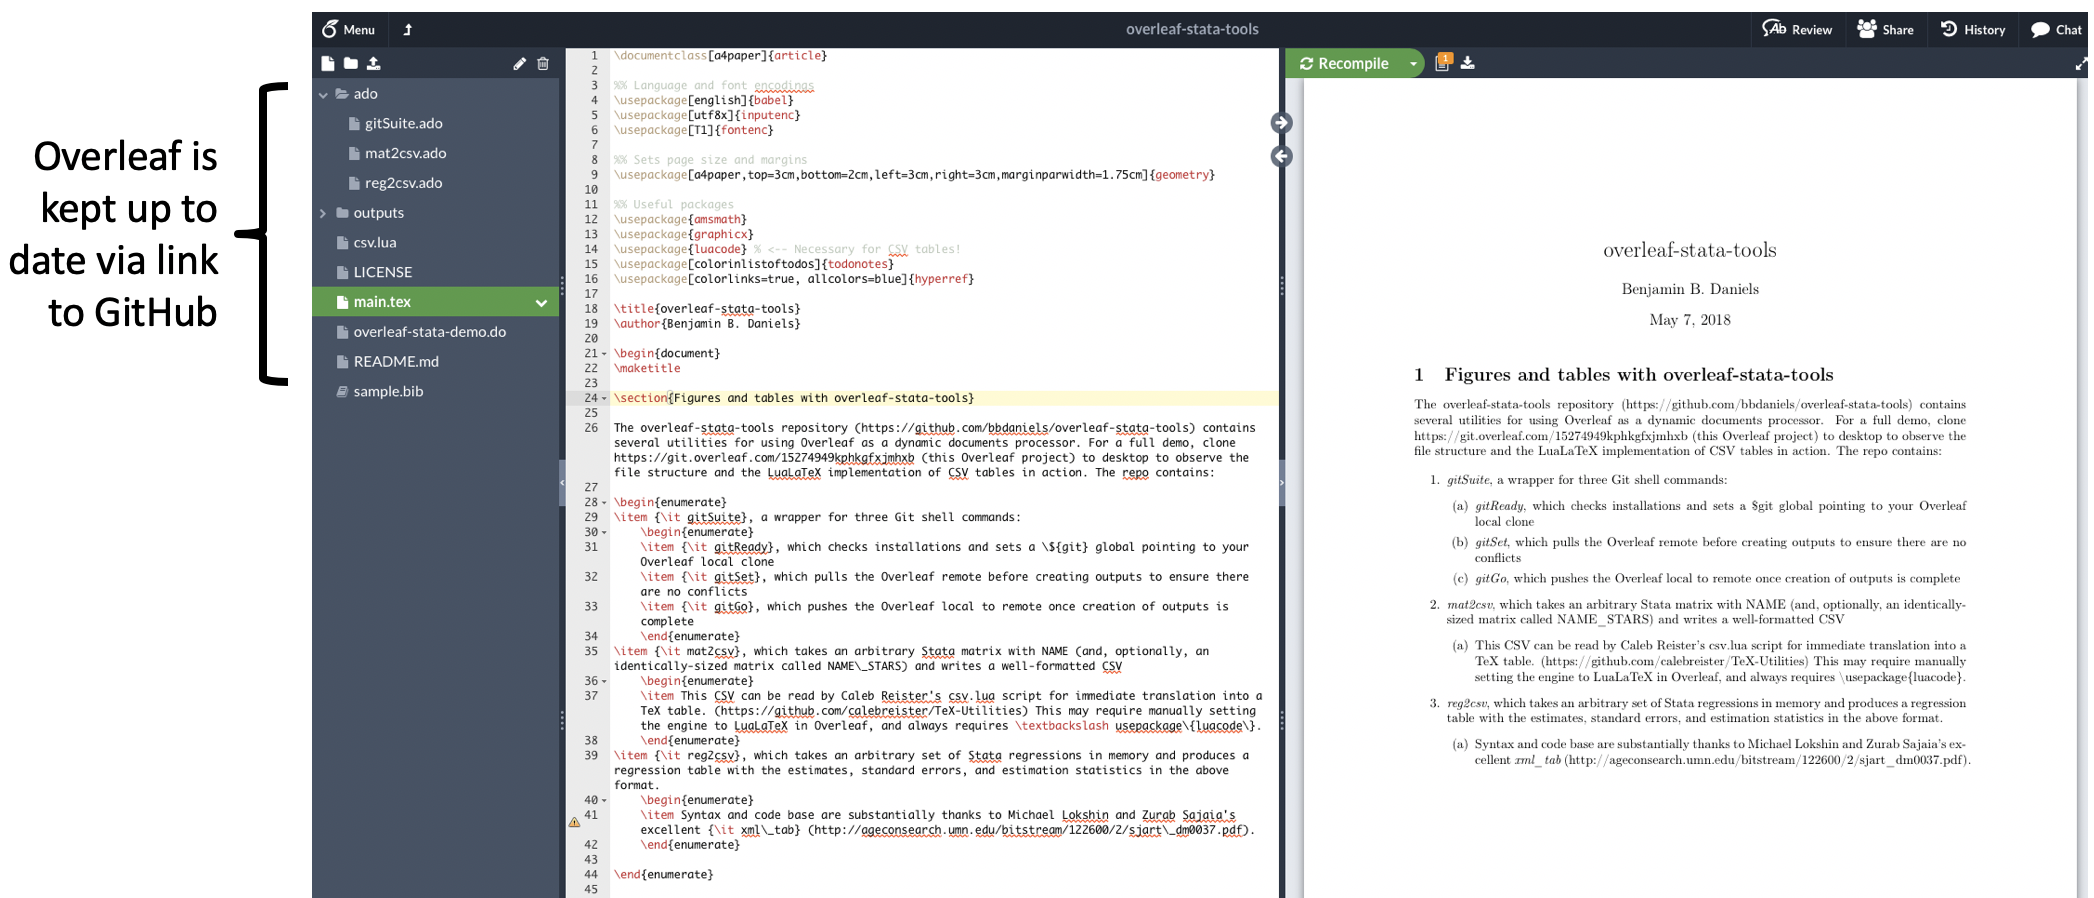
\includegraphics[width=\linewidth]{img/Writing}
\end{figure}
\end{frame}


\begin{frame}[fragile]{Publication: Public Release of Data + Code}
\begin{multicols}{2}	
	
	\textbf {Writing code on Git with collaboration public release in mind prepares the project for preservation and open access.}
	
	\begin{itemize}[<default overlay specification>]
		\item<1> The version history answers seminar questions that start with “what happened when you tried….?.”
		\item<1>  The final repository has reusable code that other projects will benefit from.
		\item<1>  Picking up the same project to extend or replicate analyses later is a one-click process. 
	\end{itemize}
	
	\begin{figure}
		\centering
		
\includegraphics[width=65mm, right]{img/Structure4}
	\end{figure}
	
\end{multicols}
\end{frame}




%%%%%%%%%% heading of section 3 %%%%%%%%%%%%%%%%%%
\sectionpic{Stata Coding: Syntax}{img/section_slide}


\begin{frame}{Stata syntax is the language of your code}
\begin{multicols}{2}	

	\begin{itemize}[<default overlay specification>]
	\item<1>  Stata code is a script, not a program.
	\item<1>  Think of a play: 
					\newline - You can read the script and get a good idea of what will happen when the instructions are followed.
					\newline - This is as important as the actual production (output) because it serves as a record of what you did.
	\item<1>  Someone is going to want to read your code!
					\newline - They want to see exactly how you got to the results.
					\newline - They want to do something similar but not identical in their own work. 
	\item<1>  More technical details:
					\newline - Stata does not work like most (“object-oriented”) programming languages.
					\newline - These (including R) treat “objects” or “functions” as the fundamental thing that is referenced by code.
					\newline - Stata is a scripting language for econometrics: its basic elements are observations and characteristics (what you know as variables but a programmer will not understand). 
	\end{itemize}

\end{multicols}
\end{frame}


\begin{frame}{Functional syntax}
\begin{multicols}{2}	
	
	\begin{itemize}[<default overlay specification>]
		\item<1>  \textbf {``Stata quotes’’}
			\newline - Will break lots of programming tools because the backtick ` is a special character.
			\newline - Are really important to get right. 
			\newline - `NAME’ calls a local macro.
			\newline - local NAME ”STRING” stores STRING in `NAME’. 
			\newline - local NAME `” “STRING” “’ stores “STRING” in `NAME’. 
			\newline - local NAME `=2+2’ stores 4 : this works anywhere, like yline(`=`beta’*`r(mean)’’).
		\item<1>  \textbf {``Equals sign =’’}
			\newline - When used with a macro, they evaluate what comes after
			\newline - local NAME = min(2,3,4) stores 2 in `NAME’
			\newline - local NAME = “min(2,3,4)” stores min(2,3,4) in `NAME’
		\item<1>  \textbf {Backslash "[/]"}
			\newline - never use in filepaths: /users/dropbox/
			\newline - “Escapes” functional characters:
			\newline - local NAME = “\`OTHERNAME’” stores `OTHERNAME’, not the contents of the local `OTHERNAME’
	\end{itemize}
	
\end{multicols}
\end{frame}

\begin{frame}[fragile]{Macros: `local’ and {global}}
\begin{multicols}{2}	
	
	\begin{itemize}[<default overlay specification>]
		\item<1> “Macros” (this is what programmers call “variables”) hold information within a Stata session.
		\item<1>  Difference in scope – Use them appropriately according to scope.
		\item<1>  Only define globals in the master do-file.
		\item<1>  Use locals everywhere else (varlists, loops, estimation results)… they are deleted after the dofile finishes. 
	\end{itemize}
	
	\begin{figure}
		\centering
		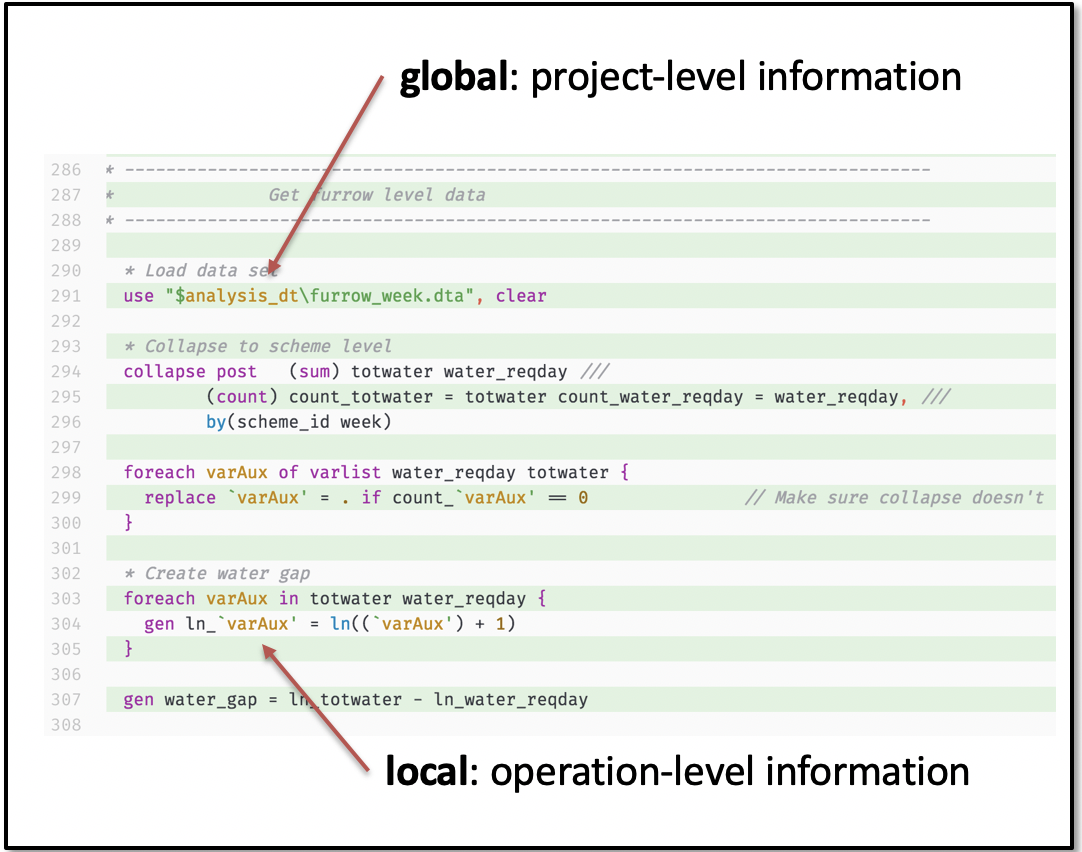
\includegraphics[width=65mm, right]{img/Syntax}
	\end{figure}
	
\end{multicols}
\end{frame}

\begin{frame}[fragile]{Macros: naming convention}
\begin{multicols}{2}	
	
	\begin{itemize}[<default overlay specification>]
		\item<1> “Always give a local or a global a name where the reader can tell what it represents.
		\item<1>  Especially in loops, abstract indices can become confusing quickly!
		\item<1>  To reiterate: Stata is a scripting language, not a programming language.
	\end{itemize}
	
	\begin{figure}
		\centering
		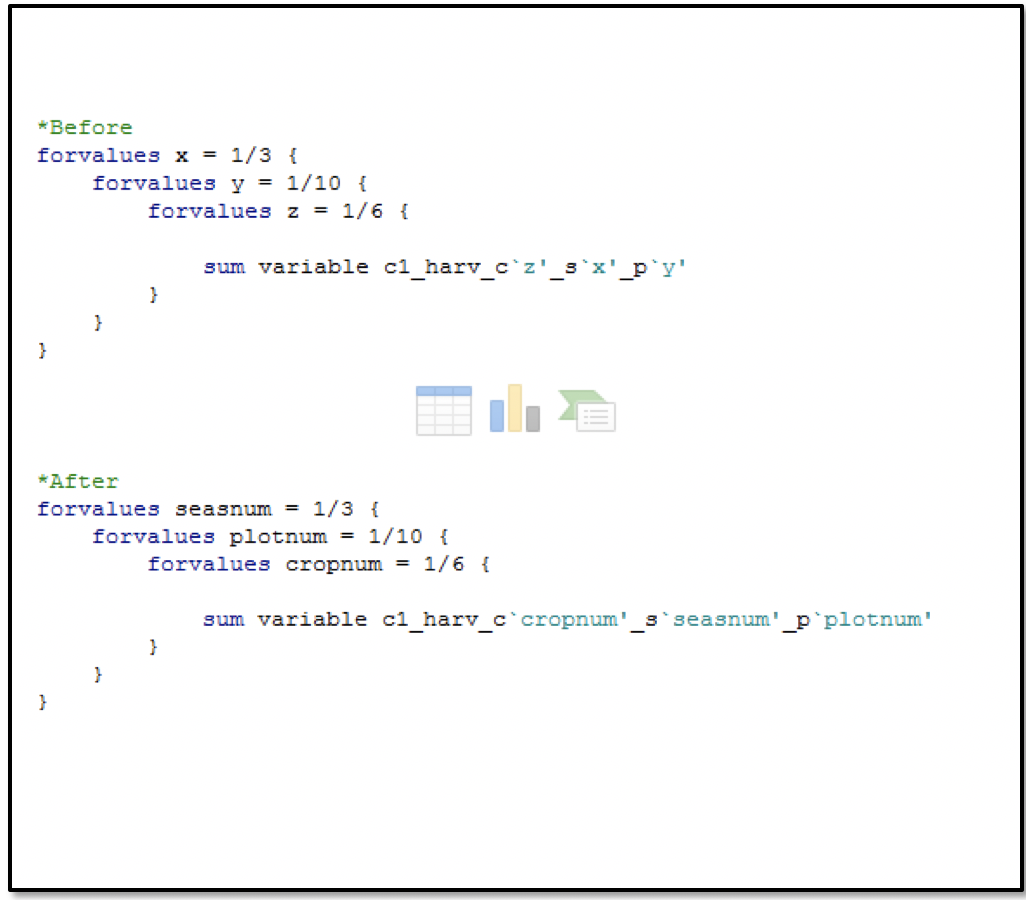
\includegraphics[width=65mm, right]{img/Syntax2}
	\end{figure}
	
\end{multicols}
\end{frame}

\begin{frame}{Tips for usages of globals}
	
	\begin{itemize}[<default overlay specification>]
		\item<1>  Only define globals in the main master do-file.
		\item<1>  Usages of globals:

			\leavevmode 	\newline  - Root folders.
			\leavevmode 	\newline  - Standardize conversion coefficients.
			\leavevmode 	\newline  - Varlists commonly used across the project – for example list of controls included in multiple regressions.
	\end{itemize}
	
\end{frame}


\begin{frame}{Tips for usages of globals}

Use locals to shorten variable names and make them more explanatory.

	\begin{figure}
	\centering
	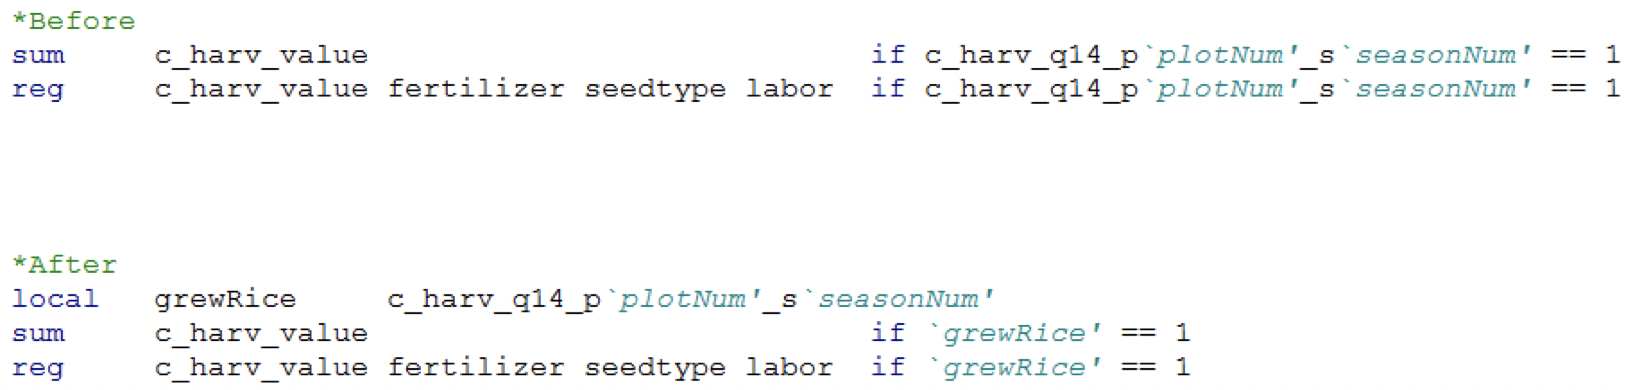
\includegraphics[width=90mm]{img/Tips}
\end{figure}

\end{frame}


\begin{frame}[fragile]{“Extended functions” in Stata}
\begin{multicols}{2}	
	
	\begin{itemize}[<default overlay specification>]
		\item<1>  Because variables are the core of Stata, it knows a lot about them.
		\item<1>  Extended functions access that information.
		\item<1> They pull information about variables (types, labels, etc), locals, and other Stata native objects into macros.
		\item<1>  local theLabel : val lab foreign
	\end{itemize}
	
	\begin{figure}
		\centering
		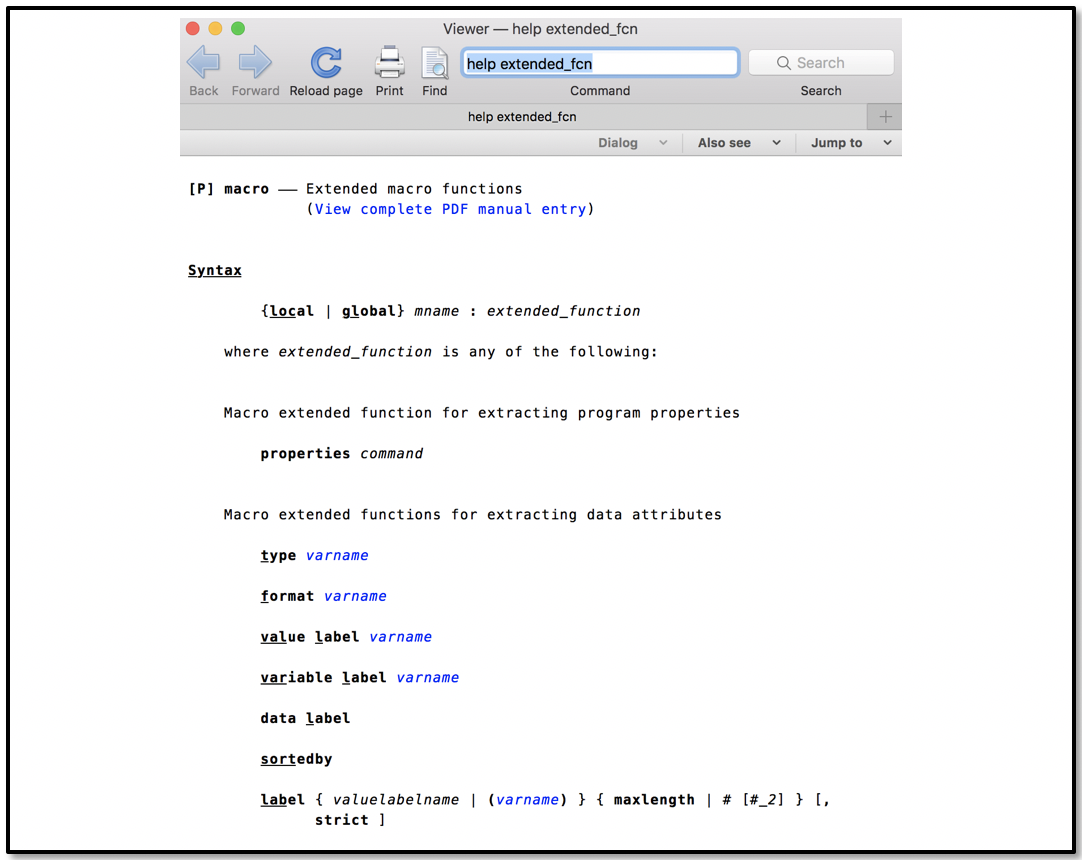
\includegraphics[width=70mm, right]{img/Tips2}
	\end{figure}
	
\end{multicols}
\end{frame}



\begin{frame}[fragile]{Stored results and [return], [ereturn], [creturn]}
\begin{multicols}{2}
	\begin{lstlisting}
	// clear
	sysuse auto
	
	// Basic Regression
	reg price mpg rep78 headroom
	local mpgBeta= _b[mpg]
	di "`mpgBeta'"
	
	*returns holds ouput
	
	return list
	
	// return list
	mat result = r(table)
	matlist results 
	
	*returns holds estimates
	
	ereturn list
	di "`e(N)'"
	count if e(sapmple) == 1
	
	*creturn holds system information
	
	creturn list 
	
		foreach letter in `c(alpha)' {
		di "`letter'" 
		}
		
	*ereturn is useful
	
	qui count
	forvalues i = 1/`r(N)' 	{
			local theName = make[`i']
			di "`theName'"
			}
	*Name a blank line at the end
	\end{lstlisting}

\end{multicols}
\end{frame}



\begin{frame}{White Space}

	\leavevmode 	\newline Stata does not distinguish between one empty space and many empty spaces, or one line break or many line breaks.
	
	\leavevmode 	\newline It makes a big difference to the human eye and we would never share a Word document, an Excel sheet or a PowerPoint presentation without thinking about white space – although we call it formatting.

\end{frame}


\begin{frame}{White space used for vertical alignment}

	\begin{figure}
		\centering
		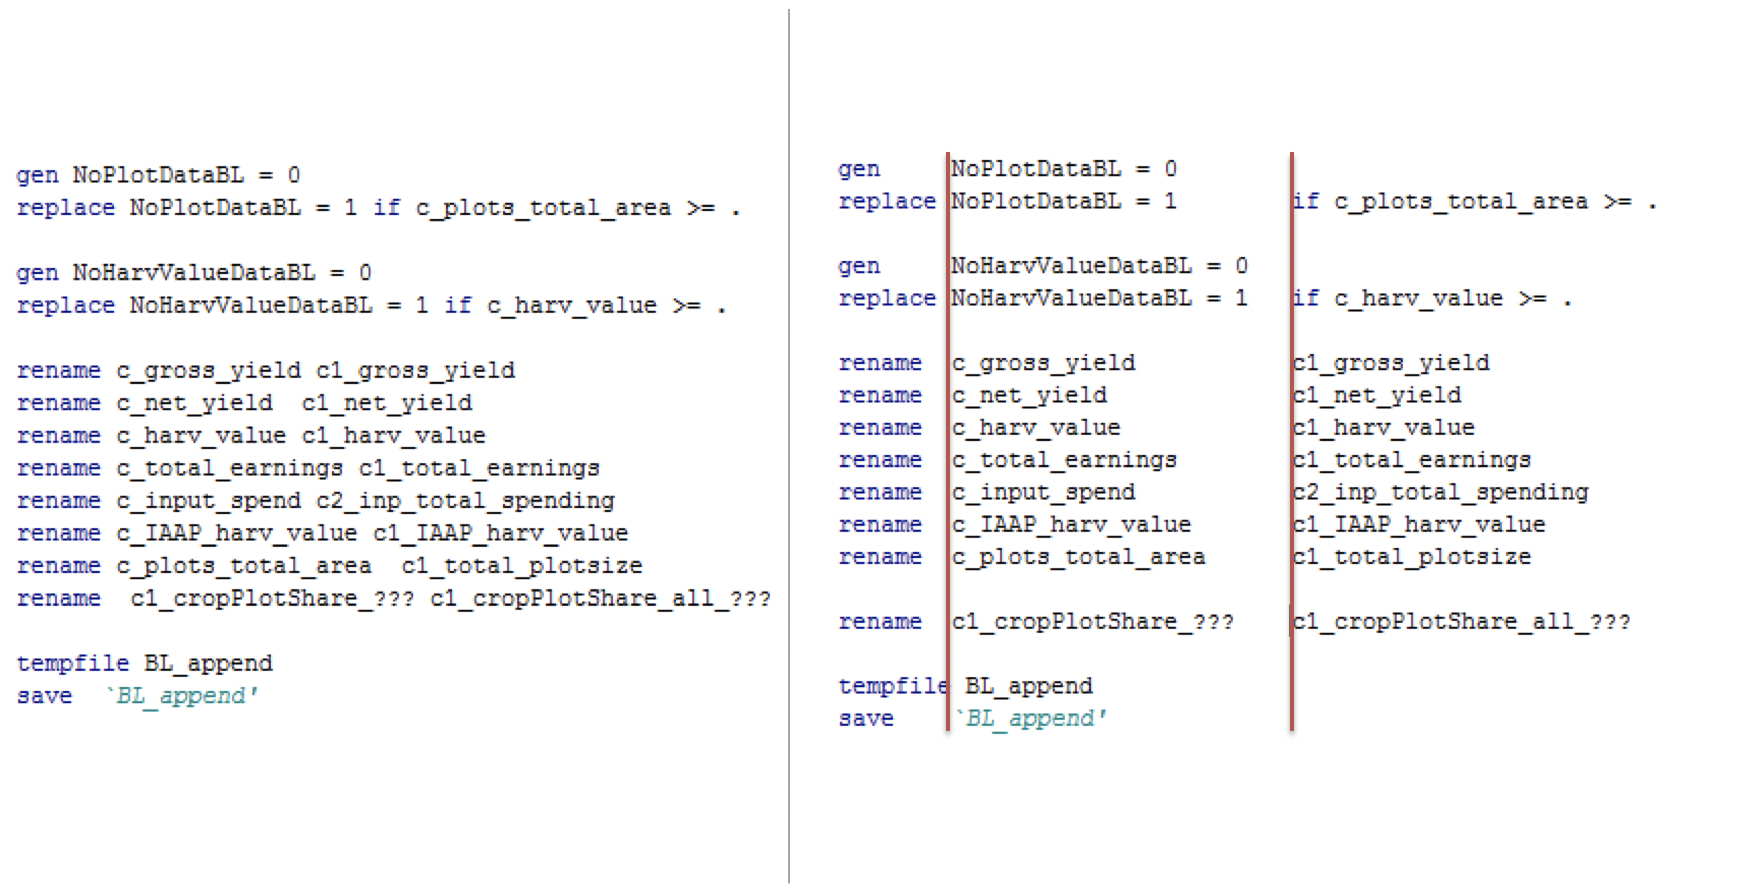
\includegraphics[width=\linewidth]{img/White_space}
	\end{figure}

\end{frame}


\begin{frame}[fragile]{White space: Indentations suggest hierarchy}
\begin{multicols}{2}	
	
	Makes code much more readable!
	
	\begin{itemize}[<default overlay specification>]
		\item<1>  Use for preserve/restore, loops and all other commands with curly brackets. 
		\item<1>  Very easy to see in “minimap” viewer (all advanced editors can display this – Atom is a particularly good one).
	\end{itemize}
	
	\begin{figure}
		\centering
		\includegraphics[width=70mm, right]{img/WHite_space2}
	\end{figure}
	
\end{multicols}
\end{frame}


\begin{frame}

	\begin{figure}
		\centering
		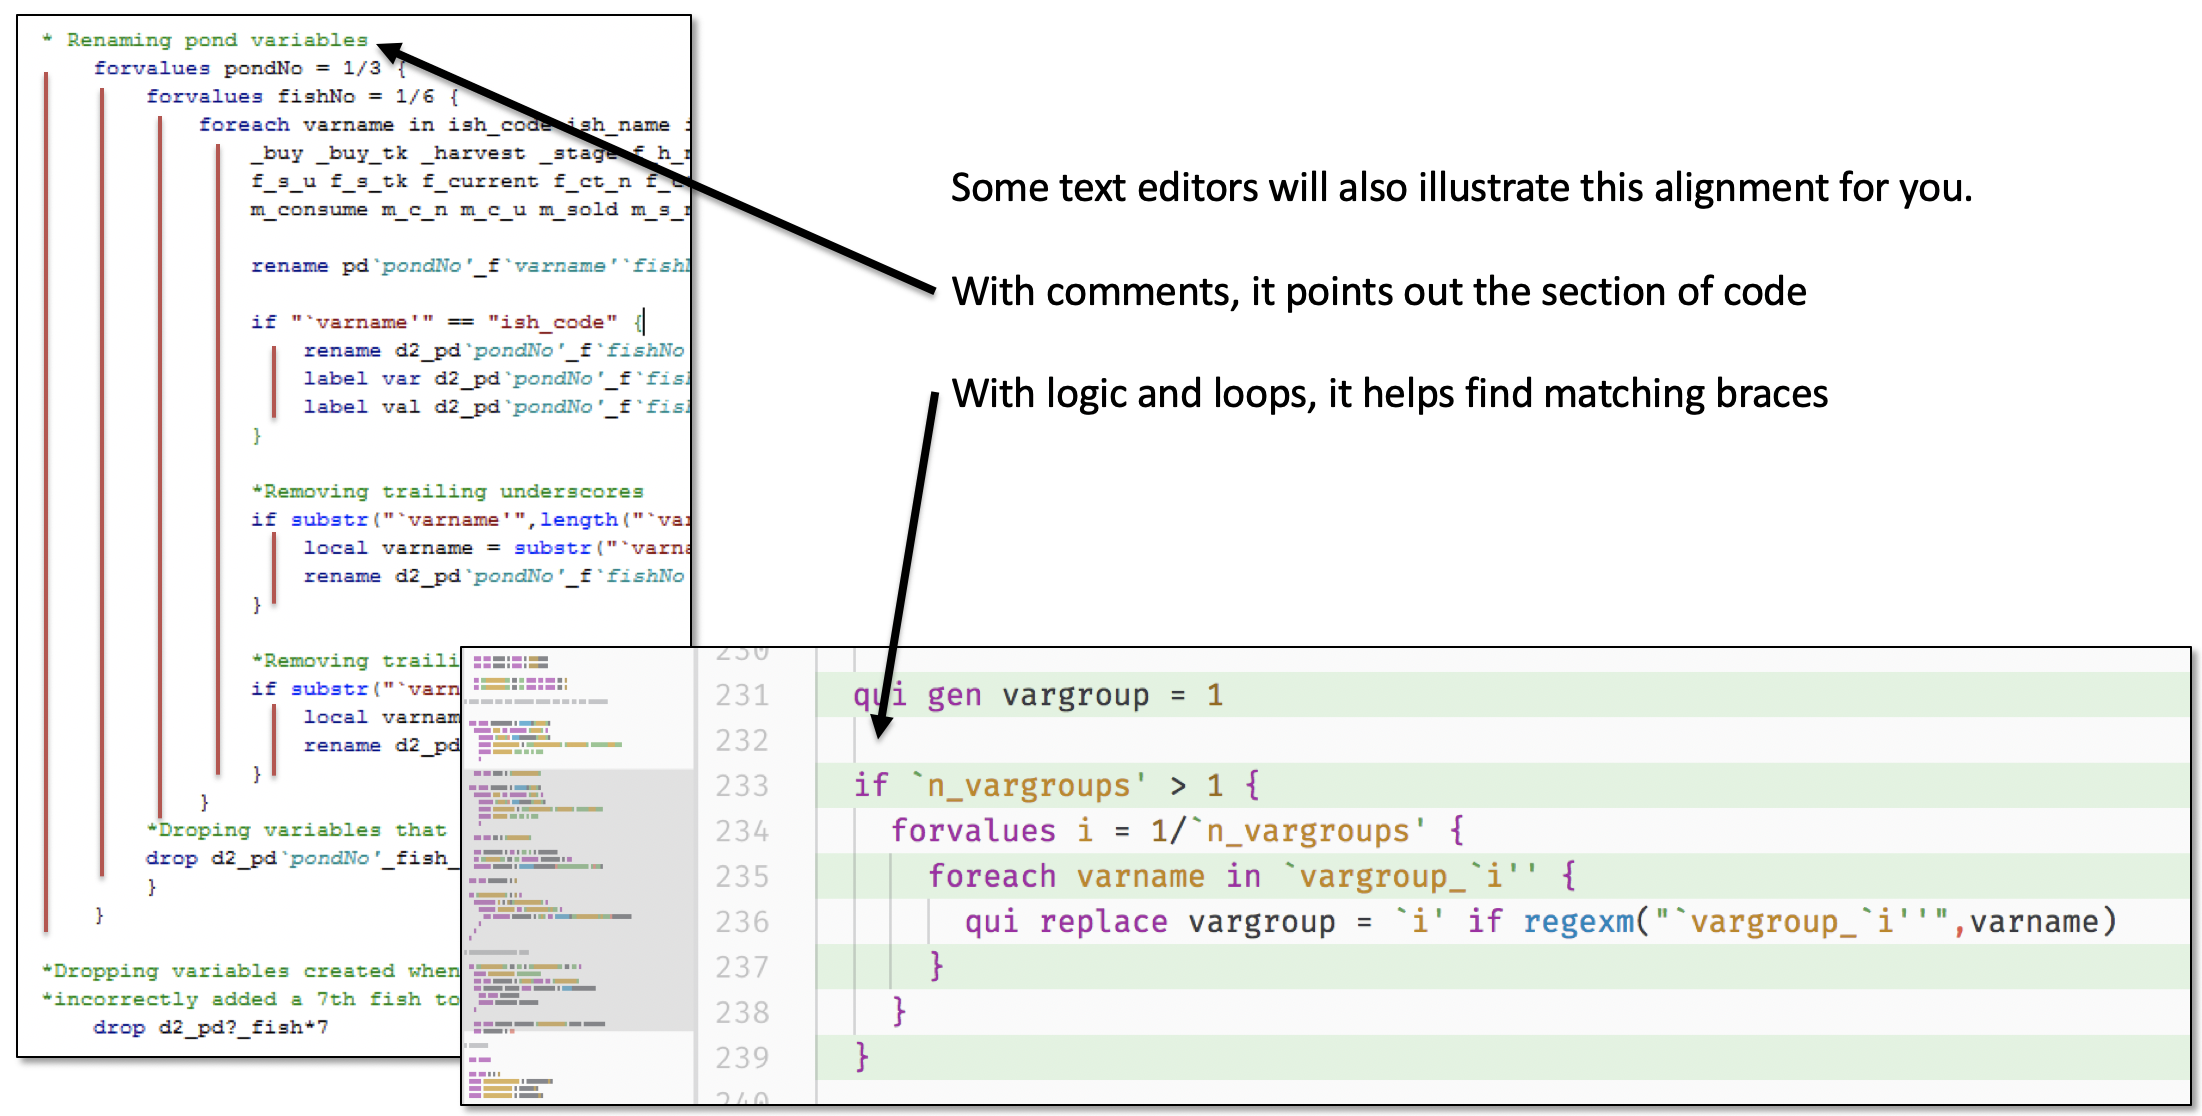
\includegraphics[width=\linewidth]{img/White_space3}
	\end{figure}

\end{frame}


\begin{frame}{Break up long rows of code}

One should never have to scroll horizontally to be able to read code
Two recommended ways to break up lines:

	\begin{enumerate}[<default overlay specification>]
	\item<1>  "///"
		\leavevmode 	\newline Everything on the same row will be interpreted as a comment and the following row will be interpreted as if it was the same row.
		\leavevmode 	\newline Good for breaking a long line of code into a few rows.
	
	\item<1>  {\#}delimit ;  and {\#}delimit cr 
		\leavevmode 	\newline Everything between {\#}delimit ; and  {\#}delimit cr is executed as one line unless it is manually specified using a semicolon.
		\leavevmode 	\newline  Good for breaking a very long line of code into many rows
	\end{enumerate}

\end{frame}


\begin{frame}{Example of row breaks}

\begin{figure}
	\centering
	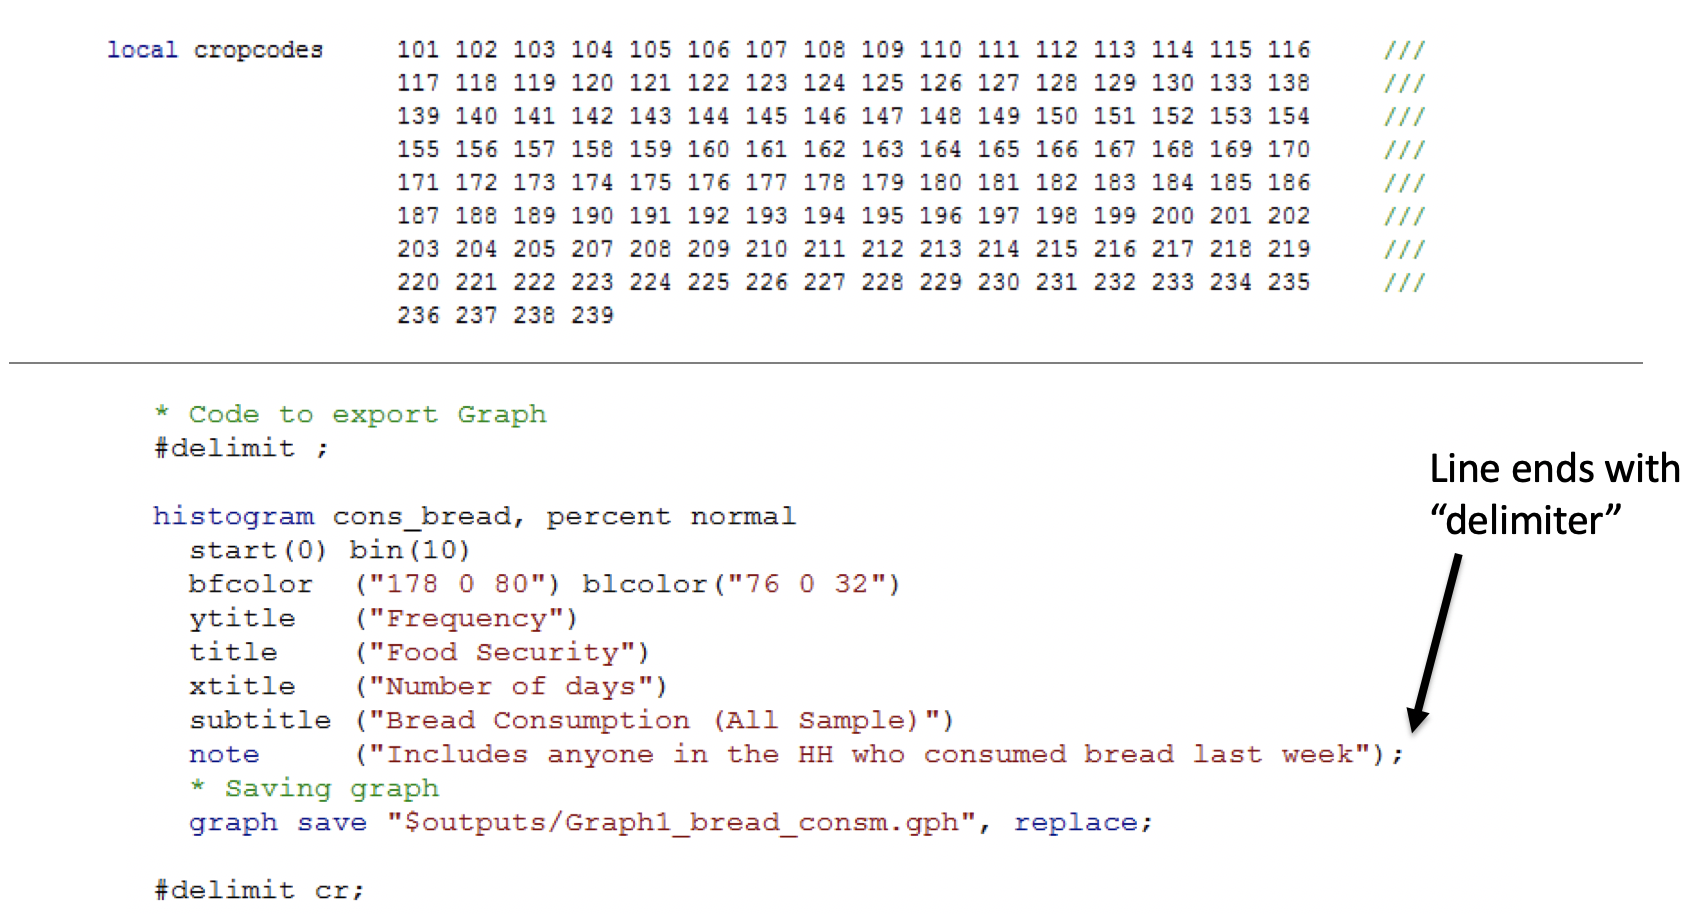
\includegraphics[width=\linewidth]{img/Row_break}
\end{figure}

\end{frame}


\begin{frame}[fragile]{Documentation is your best friend!}
\begin{multicols}{2}	
	
	\begin{itemize}[<default overlay specification>]
		\item<1>  Throughout the rest of the training sessions (and your programming life), you will need [help]!
		\item<1>  Type [help commandname] in Stata at any time.
		\item<1>  Or, google “commandname statalist” for the user-contributed help group. 
		\item<1>  Let’s read this one together:
	\end{itemize}
	
	\begin{figure}
		\centering
		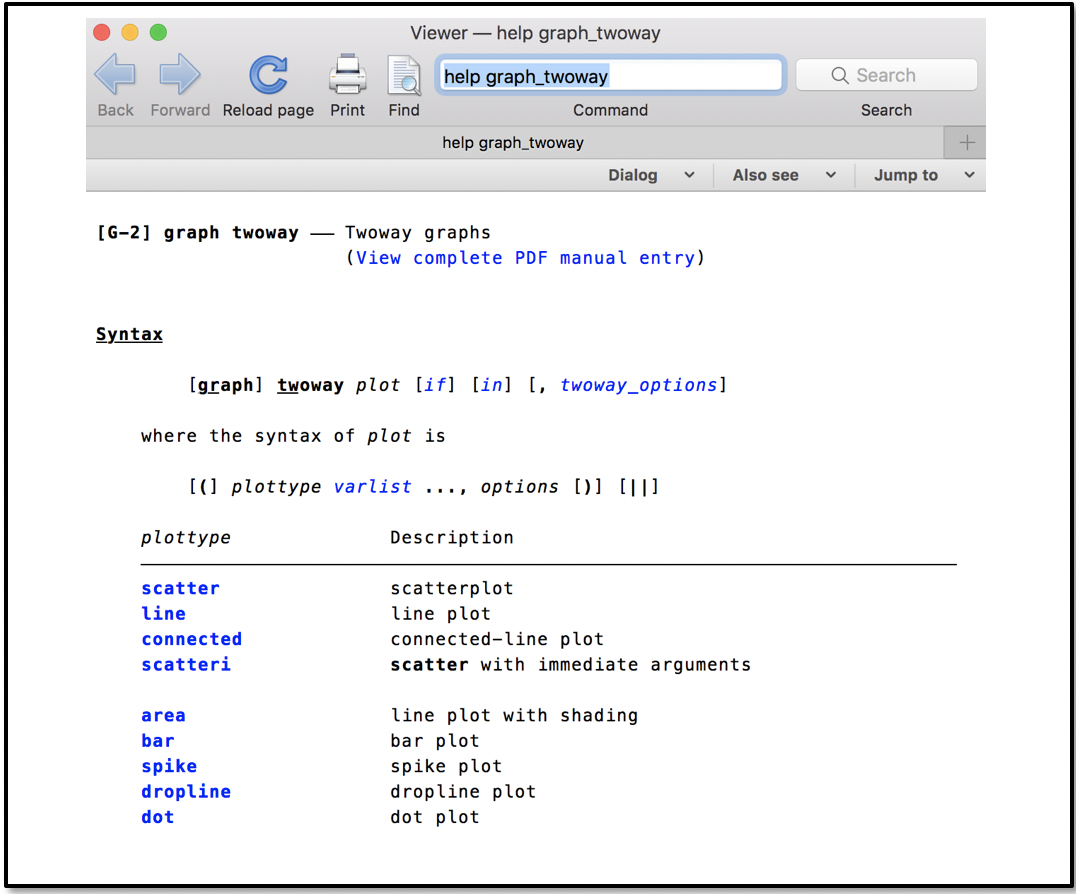
\includegraphics[width=70mm, right]{img/Help_file}
	\end{figure}
	
\end{multicols}
\end{frame}


\begin{frame}{Resources}

\leavevmode 	\newline \underline{Stata Cheat Sheets}
\leavevmode 	\newline \underline{SSC Stata Commands}
\leavevmode 	\newline \underline{UCLA Stata Tutorials}
\leavevmode 	\newline \underline{UCLA Visual Library}
\leavevmode 	\newline \underline{Stata Video Library}
\leavevmode 	\newline \underline{Speaking Stata Library}
\leavevmode 	\newline \underline{EGAP Methods Guides}

\end{frame}


\begin{frame}{Open access resources from the DIME Analytics team}

\begin{figure}
	\centering
	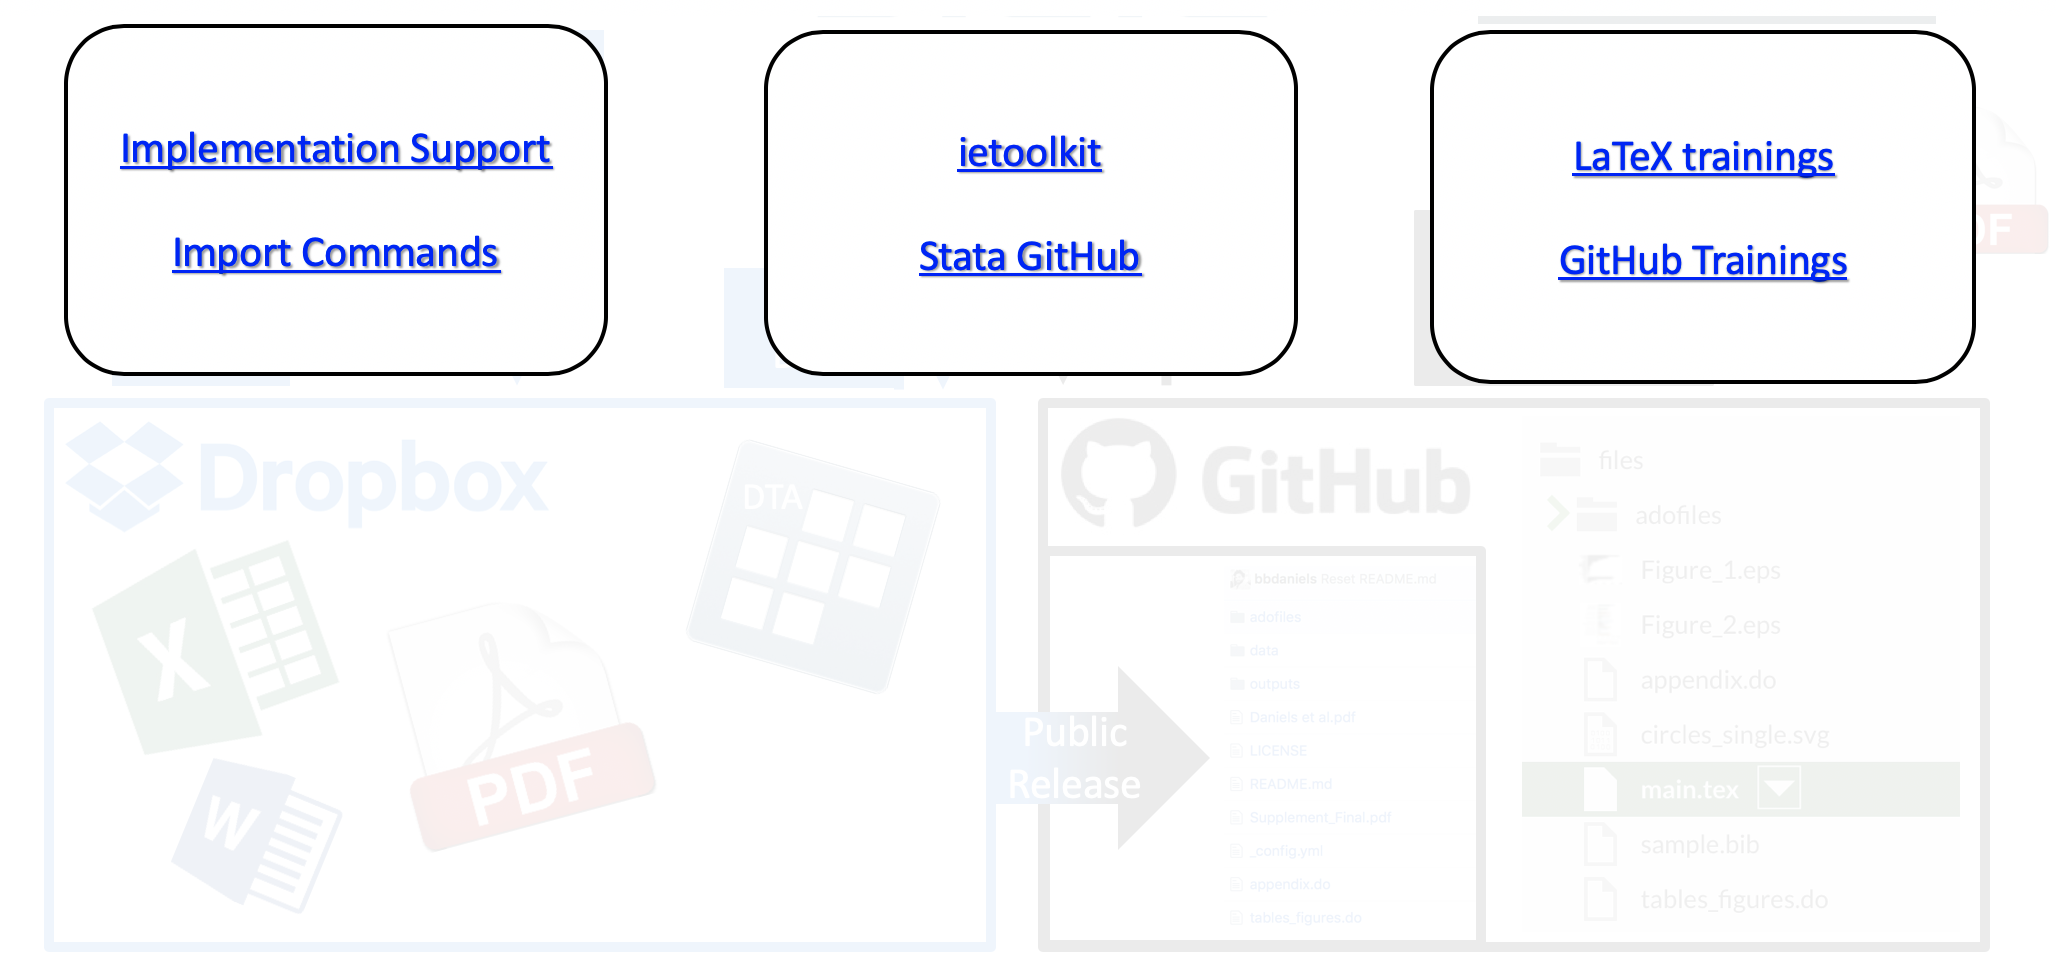
\includegraphics[width=\linewidth]{img/Resources}
\end{figure}

\end{frame}


\begin{frame}

\begin{figure}
	\centering
	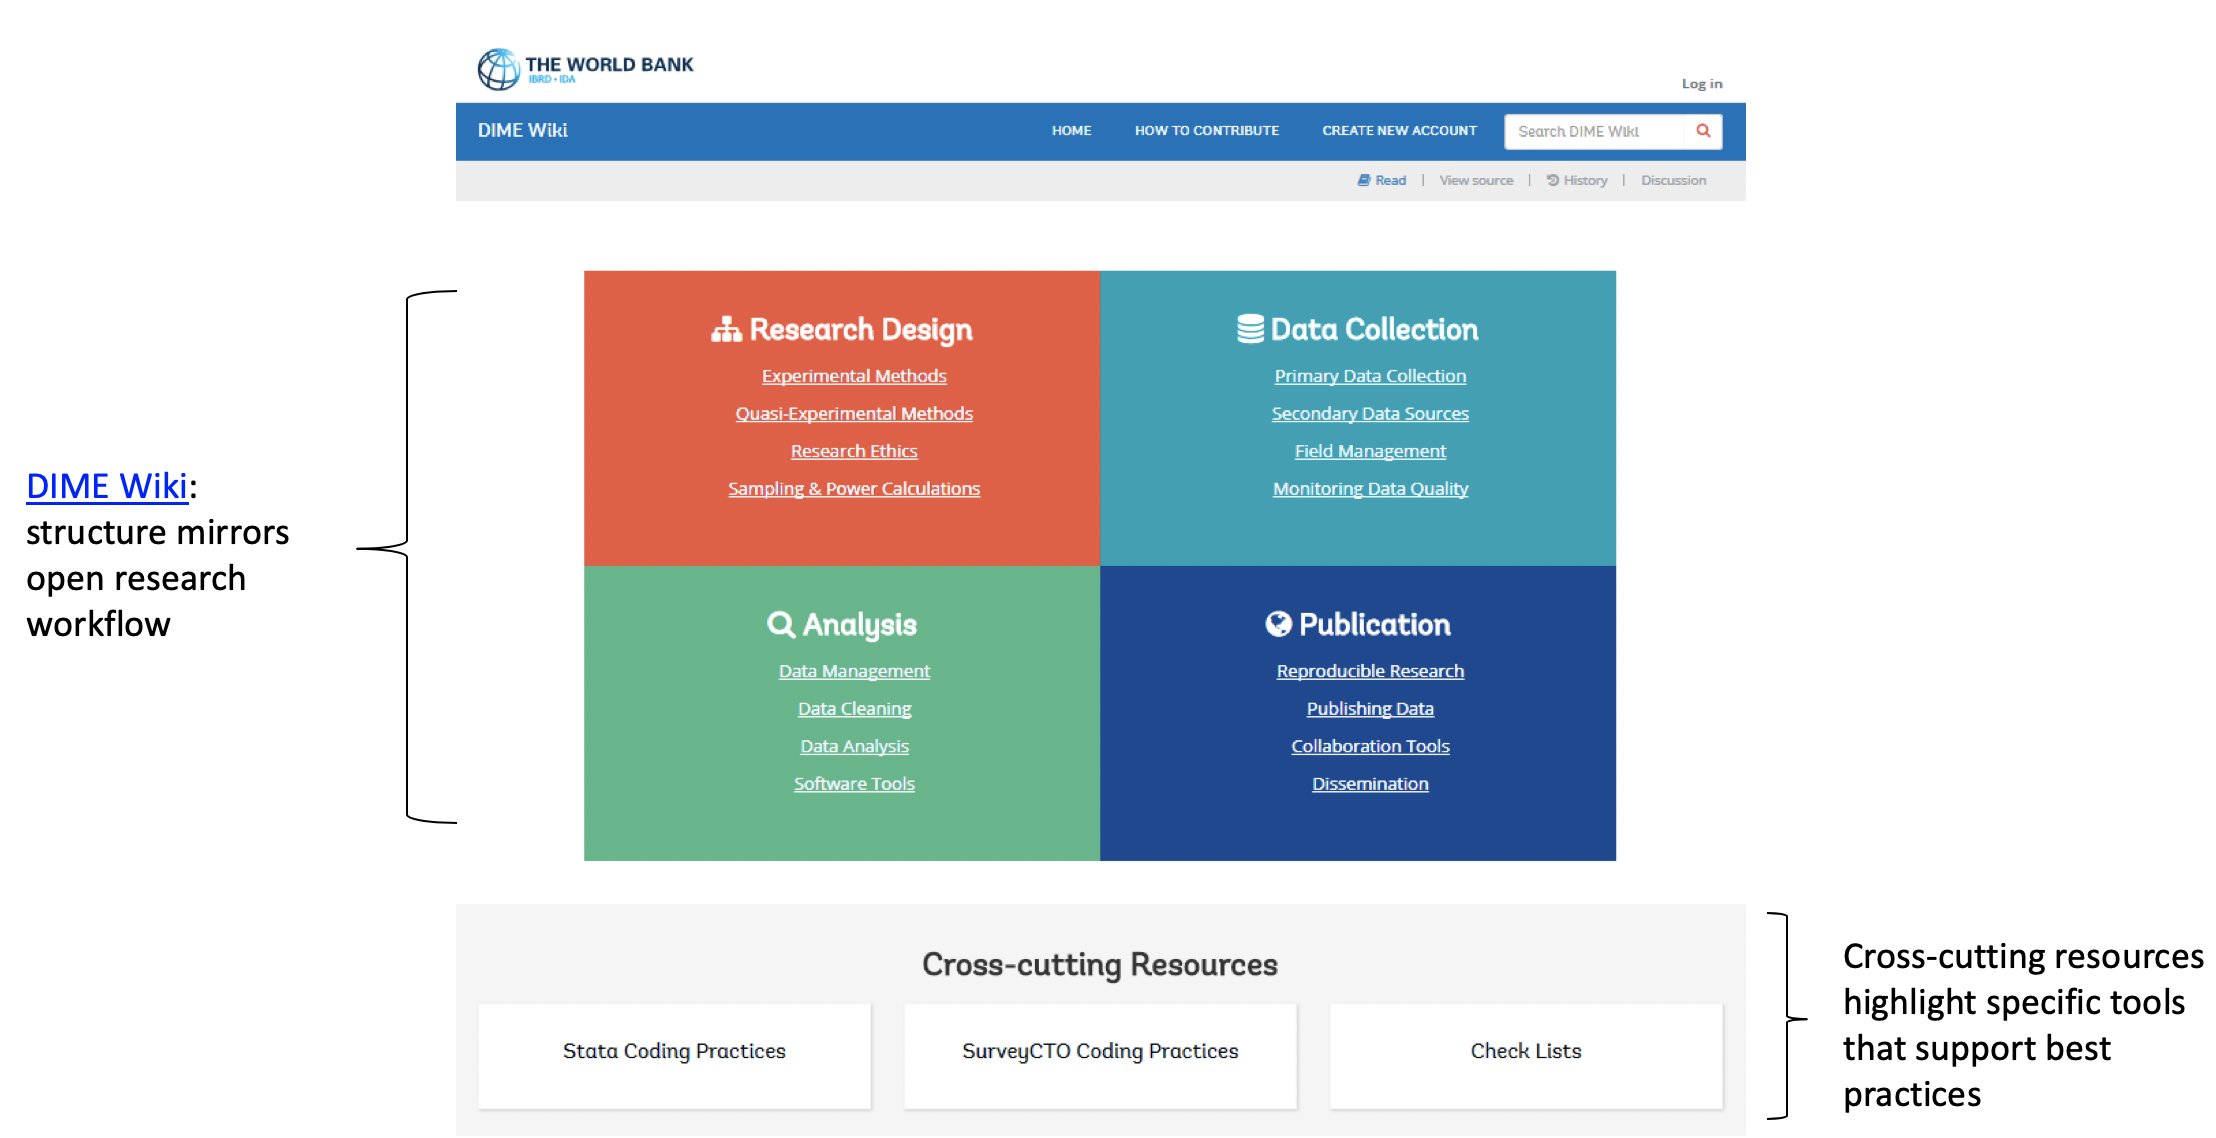
\includegraphics[width=\linewidth]{img/Resources2}
\end{figure}

\end{frame}


\begin{frame}[fragile]{World Bank GitHub Repos}
\begin{multicols}{2}	
	
Code libraries and development repositories on GitHub allow collaborative improvement of software and open-source access to researchers everywhere.
	
	\begin{figure}
		\centering
		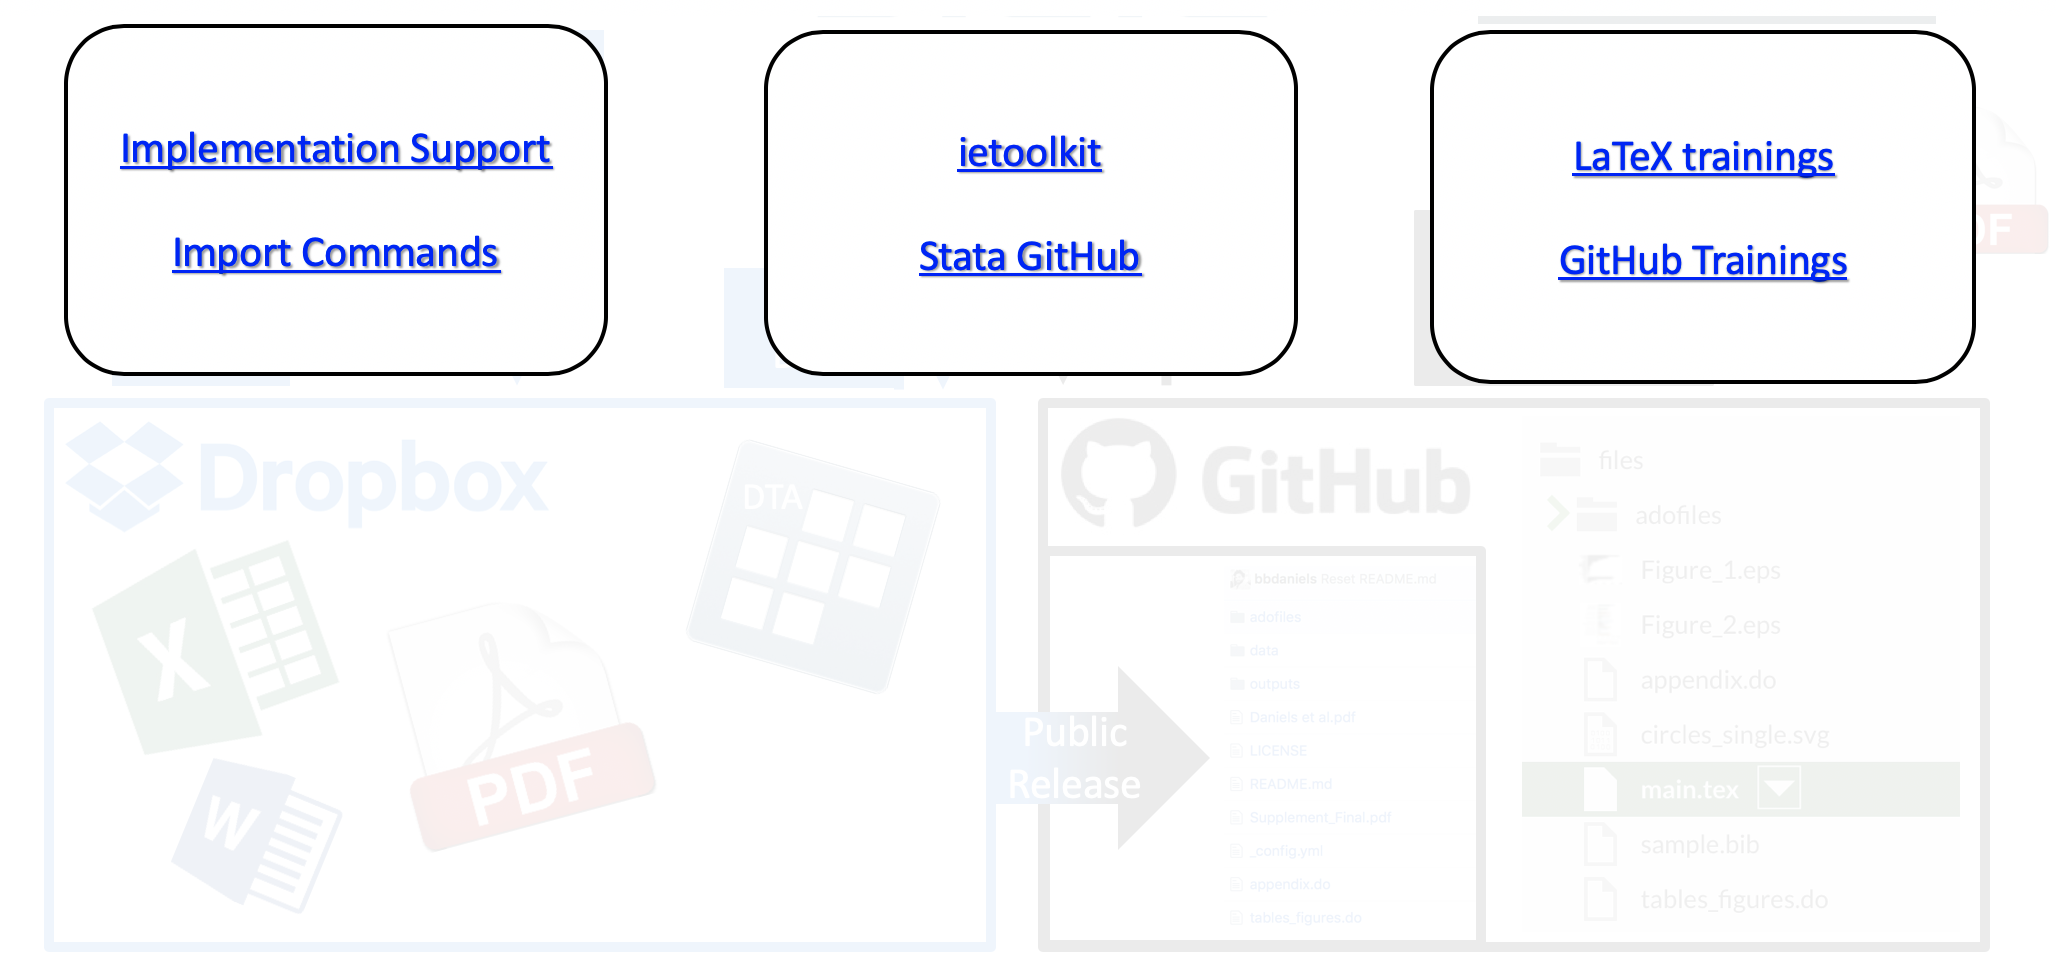
\includegraphics[width=70mm, right]{img/Resources}
	\end{figure}
	
\end{multicols}
\end{frame}

\begin{frame}[fragile]{ietoolkit}
\begin{multicols}{2}	
	
	Stata package routinizing common analytical tasks in IEs.
	
	Widely used in DIME, and endorsed by global research community.
	
	\begin{figure}
		\centering
		
\includegraphics[width=70mm, right]{img/Resources4}
	\end{figure}
	
\end{multicols}
\end{frame}

\begin{frame}[fragile]{Reproducible research tools}
\begin{multicols}{2}	
	
	\underline{LaTex}
	\newline Create dynamic documents.
	Export and update results transparently, without manual changes. 
	
	\begin{figure}
		\centering
		
\includegraphics[width=70mm, left]{img/Resources5}
	\end{figure}
	
	\underline{GitHub}
	\newline Transparent research with public codes.
	Easier collaboration.
	
	\begin{figure}
		\centering
		
\includegraphics[width=70mm, right]{img/Resources6}
	\end{figure}
	
\end{multicols}
\end{frame}

%%%%%%%%%%%%%%%%%%%%%%%%%%%%%%%%%%%%%%%%%%% Final thougts section
\begin{frame}{Conclusion}

Thank You

\vspace{20mm}
For more information or further questions please contact:
\newline Benjamin Daniels (\url{jbdaniels@worldbank.org }) 

\end{frame}

%%%%%%%%%%%%%%%%%%%%%%%%%%%%%%%%%%%%%%%%%%% The End
\sectionpic{The End}{img/section_slide}






\end{document} 